\chapter{Introduction}\label{chap:intro}

\begin{tldrbox}
	
	Monitoring the arterial \gls{co2} partial pressure---\gls{paco2}---is of paramount importance in clinical practice. The latter can be measured directly (arterial puncture) or through proxies (tracheal intubation and transcutaneous monitoring). However, current monitors suffer from a variety of drawbacks which hamper their wider use. Thus, there is an urging need for a new kind of non-invasive, low-cost, and portable---if not wearable---biomedical \gls{co2} monitor.
	
	Two main research avenues were identified to address this issue. The first one extrapolates the principle of pulse oximetry to the non-invasive determination of the arterial \gls{co2hb} content. This approach mainly focused on spectrophotometric considerations but ultimately proved to be a dead-end---it is the object of Chapter~\ref{chap:co2hb}. The second approach relies on transcutaneous \gls{co2} diffusion. It is further divided into: studying the transcutaneous \gls{co2} diffusion phenomenon itself---Chapter~\ref{chap:tcco2}---finding a \gls{co2} sensing technology compatible with it---Chapter~\ref{chap:choosing_techno}---and putting this knowledge into practice by actually designing such a transcutaneous sensor---Chapter~\ref{chap:thin_film}.
	
	\tcblower
	
	\hyperref[forechap:ack]{Previous chapter} \hfill \hyperref[chapter:toc]{Main Table Of Content (TOC)} \hfill \hyperref[chap:co2hb]{Next chapter}
	
\end{tldrbox}\glsresetall

\section{Carbon Dioxide as a Vital Sign}

As Thomas Henry Huxley argued during his 1874 lecture to the British Association\cite{huxley1874_nat} \enquote{We are conscious automata}\footnote{Actually the exact wording comes from one of his essays, published the same year\cite{huxley1874}. Over a century of scientific research have gone by, and further nails have been added to the coffins of free will and soul, Anthony Cashmore further adding that \enquote{Neither religious beliefs, nor a belief in free will, comply with the laws of the physical world}\cite{cashmore2010}.}. And if we are but machines---although highly sophisticated ones---the question that arises next when it comes to our survival is that of maintaining our operating conditions---what biologists calls homeostasis. Maintaining this homeostasis throughout the human body requires energy and generates wasteful by-products, and just as a petrol engine needs:
\begin{enumerate}
	\item some fuel (petrol) and
	\item an oxidizing agent (\gls{o2}) to produce
	\item a useful work (mechanical motion) as well as
	\item unwanted by-products that have to be disposed of (heat and exhaust gases),
\end{enumerate} 
our body needs:
\begin{enumerate}
	\item an energetic substrate (such as carbohydrates, lipids or proteins) and
	\item an oxidizing agent (also \gls{o2}) to produce
	\item a useful work (\eg{} maintaining homeostasis, moving, breeding) as well as
	\item unwanted by-products that have to be disposed of (heat, \gls{co2}, and various excreta)
\end{enumerate}

Medicine, which may be defined as \enquote{the process of enabling people to increase control over, and to improve their health}\cite{who_health_glossary_2021}, aims at maintaining homeostasis as long as possible. To this end, the monitoring of so-called \emph{vital signs}---blood pressure, temperature, pulse rate and respiratory rate\cite{lockwood2004}---is of crucial importance to ensure that no illness or injury impedes the normal functioning of the body. In addition to these four traditional vital signs, pulse oximetry\cite{callahan2008}, end-tidal \gls{co2}\cite{ahrens2004, hunter2014}, walking speed\cite{middleton2015} or pain\cite{morone2013} have all been proposed as supplementary fifth (or sixth) vital sign by a number of authors. These auxiliary variables, along with others---\eg{} arterial blood glucose level or bicarbonate ion concentration---make up the set of \emph{physiological parameters}, whose monitoring can give the clinician valuable clues about their patient's state.

% About secretin, see Chey2014, "Secretin Historical Perspective and Current Status", DOI: 10.1097/01.mpa.0000437325.29728.d6

The choice of which parameter to monitor heavily depends on the patient's physiology, and the provided information varies considerably from one parameter to another, some parameters being very sensitive but not very specific---\eg{} heart rate---while others are very specific, but harder to monitor---\eg{} secretin plasma concentration. Among them, blood gases---namely \gls{o2} and \gls{co2}---and their arterial partial pressures (\gls{pao2} and \gls{paco2}) give respiratory as well as circulatory clues on the state of a patient\cite{wagner2015}. This latter characteristic is particularly valuable given that, according to the \gls{who}, three of the six leading causes of death worldwide are related to respiratory diseases, as illustrated in Figure \ref{fig:who_causes_death}. As an example, \gls{copd} has been shown to entail a significant increase in \gls{paco2} combined with a decrease in \gls{spo2}\footnote{\gls{spo2} is the name given to the \gls{o2sat} when measured by pulse oximetry---Section~\ref{sect:co2hb:pulse_oximetry}. \gls{o2sat} and \gls{pao2} are linked together by the oxygen–haemoglobin dissociation curve \aka{} \enquote{Barcroft curve} from the name of Joseph Barcroft, the British physiologist that discovered it\cite{barcroft1909}. \gls{spo2} is thus often used as a proxy for \gls{pao2} in a clinical setting, given its ease of measurement compared to an arterial puncture\cite{nitzan2014, jubran2015, tamura2019}, as discussed below---see Section~\ref{subsect:co2hb:o2_transport}.} along the course of its progression\cite{cukic2014, rajeh2016}. It has further been shown that \gls{paco2} is a good predictor of survival and hospitalisation rates in \gls{copd} patients\cite{nava1994, kessler1999, park2006}, as well as in other pathologies---\eg{} tuberculosis\cite{tsuboi2010} or pulmonary embolism\cite{ozsu2012}. Thus, the continuous monitoring of \gls{paco2} is of paramount importance in medical practice, especially for patients presenting severe respiratory disorders.

\begin{figure}
	\centering
	\includegraphics{1_main_matter/intro_figures/tikz/out/who_bargraph}
	\caption[The ten leading causes of death according to the WHO.]{The ten leading causes of death worldwide, according to the latest \gls{who} report (2019)\cite{who_causes_death_2019}. Three out of ten---in red---concern respiratory-related diseases, which accounted for 13.7\% of deaths worldwide in 2019.}
	\label{fig:who_causes_death}
\end{figure}



\section{\texorpdfstring{\gls{co2}}{CO2} Sensing in Medical Practice}

As a by-product of aerobic metabolism, \gls{co2} is ubiquitous in human body, and its influence on pH makes its regulation in the organism a key parameter to maintain homeostasis\cite{jones2008}. In particular, \gls{co2} equilibrium is controlled by several mechanisms governing the efficiency of gas exchange\cite{guyenet2015, nunnschap5} and by renal regulation of plasma bicarbonate ions\cite{hamm2015}. Both the excess or deficiency of \gls{co2} in the organism---termed hyper- and hypocapnia, respectively---can have either beneficial or deleterious effects on a patient's outcome, depending on their condition\cite{curley2010}. As a consequence, \gls{co2} monitoring is of major importance in clinical care. Its measurement can be performed in three locations, presented in order of decreasing invasiveness:

\begin{enumerate}
	\item	inside the body with blood or tissues sampling---Section \ref{subsect:bloodgasanal},
	\item	in the exhaled air with airway capnometry---Section \ref{subsect:airway_cap},
	\item	on the skin with transcutaneous capnometry---Section \ref{subsect:transcut_capno}.
\end{enumerate}

An illustration of these locations is provided in Figure \ref{fig:three_probing}. For each one of them, the clinical significance of the corresponding \gls{pco2} measurement is first presented, and its probing modalities in practice are then described. One should bear in mind through the remainder of this section that \gls{co2} transport in the human body takes three distinct forms: dissolved \gls{co2}, bicarbonate ions, and carbamate compounds\footnote{This aspect is further detailed in the \hyperref[chap:co2hb]{next chapter}.}. Those are in constant equilibrium for a given blood pH, and could give rise to as many measurements---blood \gls{pco2}, $[HCO_3^-]$, \gls{co2hb} concentration and pH\cite{geers2000, nunns}. Yet, for both practical and physiological reasons, \gls{pco2} measurements have been predominantly adopted from a clinical perspective.

\begin{figure}
	\centering
	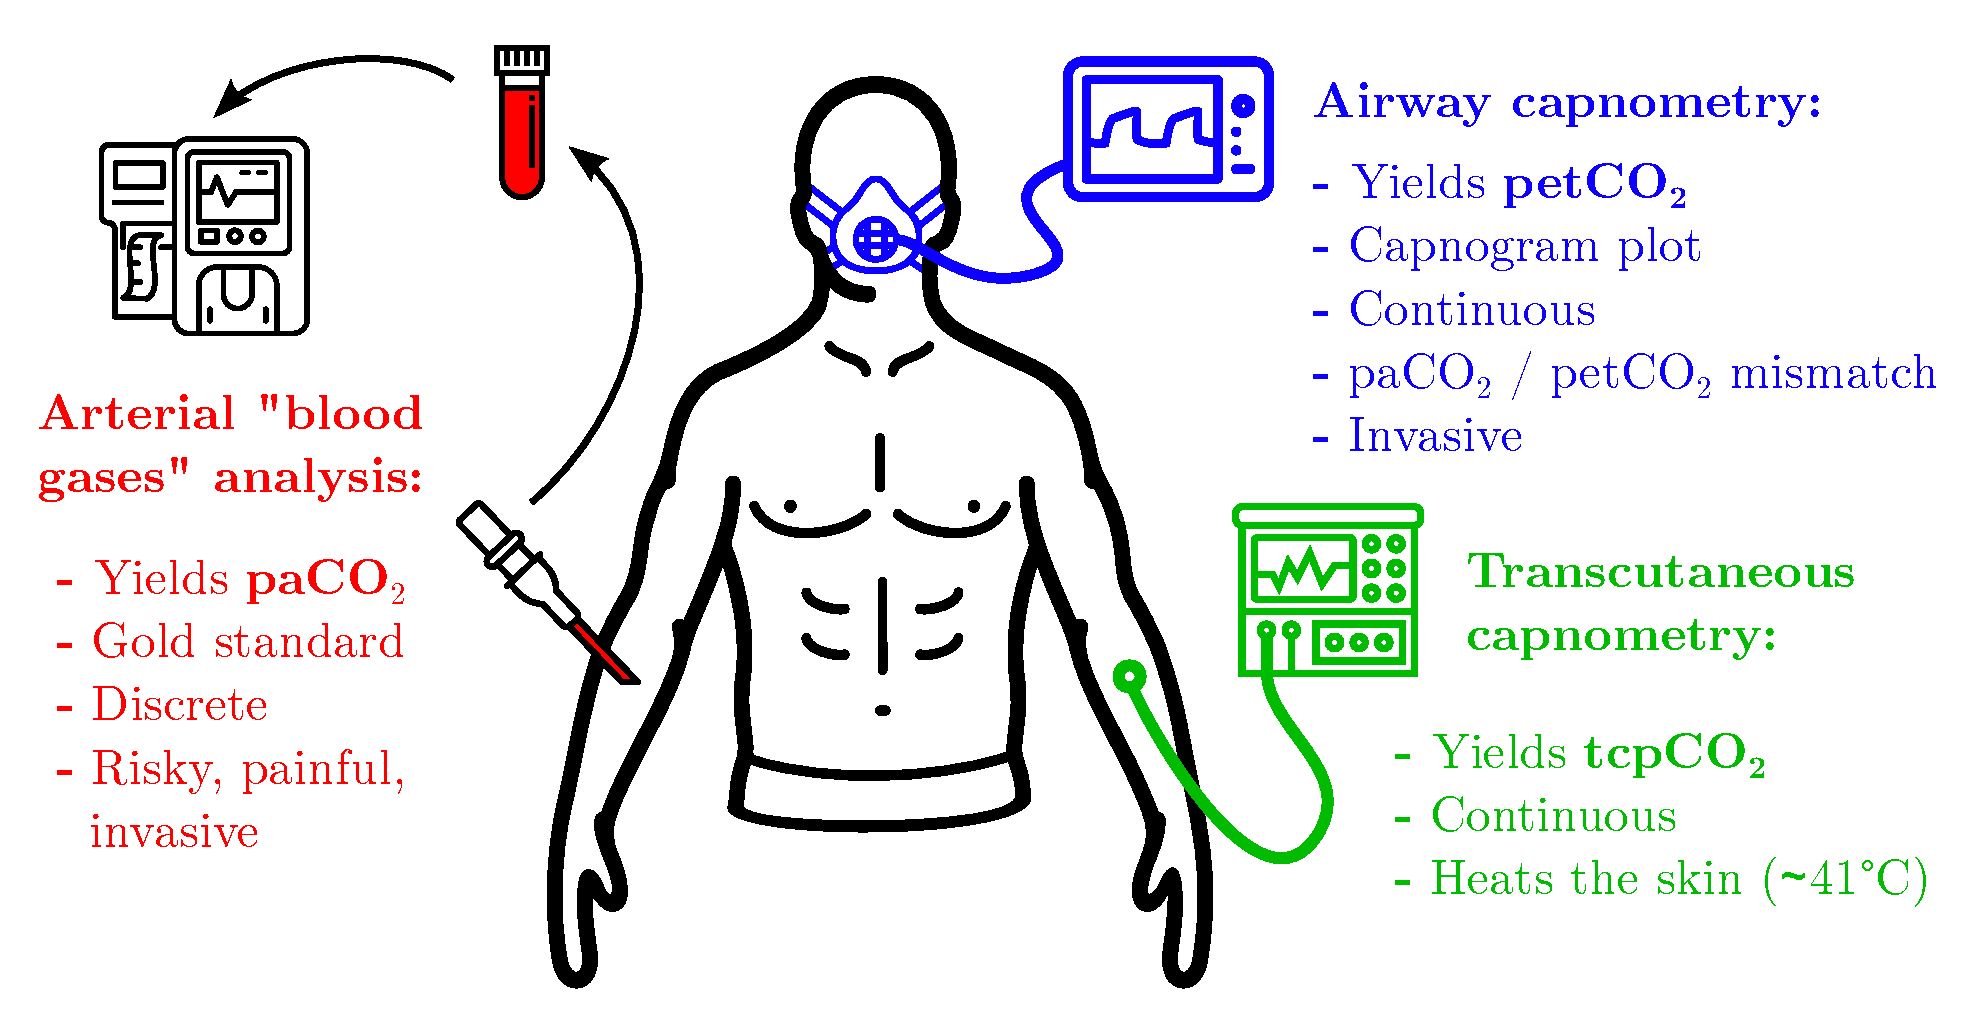
\includegraphics[width=.99\linewidth]{1_main_matter/intro_figures/sensors_capno_principle}
	\caption{The three \emph{in vivo} \gls{co2} probing modalities and their key features.}
	\label{fig:three_probing}
\end{figure}

\subsection{Blood Gas Analysis}\label{subsect:bloodgasanal}

\subsubsection{Clinical Significance}\label{subsect:bloodgas_sig}

Arterial blood sampling is considered to be the gold standard for the assessment of whole-body \gls{co2} content. Arterial blood exits the lungs without perfusing any organ. Contrary to capillary or venous blood, it is thus fully oxygenated with a low \gls{co2} content, and is not impacted by the activity of the organ that it perfuses\cite{kowalchuk1988, diaztagle2017}---see Section \ref{subsect:tcco2:frontiers:acc_impact}. Consequently, the arterial partial pressure in \gls{co2}---\gls{paco2}---best represents the global haemodynamic status of patients, and gives important clues about their metabolism and homeostasis\cite{larkin2015, wagner2015}. There is an extremely large panel of clinical applications for \gls{paco2} measurements, including acute and chronic respiratory failures\cite{foster1988, cukic2014}, mechanical ventilation assessment\cite{nava1994, tsuboi2010}, general anaesthesia---but also sedation in patients at risk of hypoventilation---monitoring\cite{campbell1994}, or resuscitation procedures\cite{schneider2013}. Due to the painful and potentially risky aspects of arterial blood puncture\cite{scheer2002}, other blood sampling techniques have been explored. In particular, arterialised capillary blood sampling was reported to be an acceptable surrogate for arterial blood sampling\cite{zavorsky2007}. In contrast, peripheral venous blood cannot be used to this end\cite{byrne2014}, nor can central venous blood\cite{malinoski2005, treger2010, walkey2010}, even if both may be used for trend analysis. Venous blood \gls{pco2} measurement is nevertheless interesting in critically ill patients, for whom measuring the venous-to-arterial carbon dioxide partial pressure difference (\gls{pvaco2})---or calculating the venous-to-arterial carbon dioxide content difference---makes it possible to detect organ hypo-perfusion\cite{scheeren2018}.

% LOA for central venous (mmHg?)
% treger : -12.3 -- 4.8
% walkey : -7.5 -- 6.5
% malinoski : -2.2 -- 10.9

More localised \gls{pco2} measurements have also been performed with intra-tissue probing---in particular into the brain\cite{charbel2000}, liver\cite{brooks2007} or skeletal muscles\cite{mckinley1999}---yielding crucial information about the perfusion of the organ under study. Gastric tonometry and sublingual capnometry have also been explored, but their clinical interest have yet to be fully demonstrated\cite{mythen2015, mallat2018}.

% On gastric tono:
% 10.1097/00003246-200003000-00001
% 10.1186/s13054-015-0739-6 (Zhang)

\subsubsection{Probing Modalities}

\textit{In vivo} \gls{co2} probing can be achieved under two distinct modalities. Either \gls{pco2} is measured \textit{in situ} or a biological sample is collected to be further analysed.

In the first case, the sensor is brought to the analyte. This is notably what happens for intra-tissue \gls{pco2} monitoring. In such cases, the sensor is inserted directly into the organ or blood vessel that is to be probed by means of a catheter, for instance. This setting allows for continuous monitoring with a low latency, which is only dictated by the response time of the chosen \gls{pco2} sensor\cite{ganter2003}.

In the second case, often used for blood \gls{pco2} measurements, the analyte is brought to an external analyser and an arterial or venous line placement may be performed to facilitate repeated blood sampling. However, this setting allows only discrete monitoring since a blood sampling must be performed every single time a \gls{pco2} is desired. In addition, the blood samples must be analysed quickly upon collection, which may lead to additional logistic difficulties compared to \textit{in situ} sensing\cite{nanji1984}, even if recent hand-held blood gas analysers tend to mitigate this issue\cite{luukkonen2016}.

In practice, two main technologies have been used to perform blood gas analysis: optodes using dye-based \gls{co2} sensing---as described in Section \ref{subsect:choos:review:dye_based}\cite{ganter2003, menzel2003}---and electrochemical sensors such as the \ssel{}---described in Section \ref{subsect:choos:review:ssel}\cite{badnjevic2011}.

\subsection{Airway Capnometry}\label{subsect:airway_cap}

\subsubsection{Clinical Significance}\label{subsect:airway_capno_cc}

Airway capnometry---from Greek \textit{capnos} ($\kappa\alpha\pi\nu o \varsigma$), smoke, vapour---is the measurement of the amount of \gls{co2} in exhaled air. Please note that there is a semantic distinction between capno-\emph{metry}---which consists in the measurement of \gls{petco2}, the end-tidal \gls{pco2}---and capno\emph{graphy}---which usually refers to the plot of a capnogram: \gls{pco2} in the exhaled air as a function of time, or volume. The distinction between capnometry and capnography is made clear in Figure \ref{fig:capnometry_principle}.\todo{refaire les (I), (II) (III) en \Circled{1}, \Circled{2}, \Circled{3}, sous TikZ? (pour cohérence taille de police)}

\begin{figure}
	\centering
	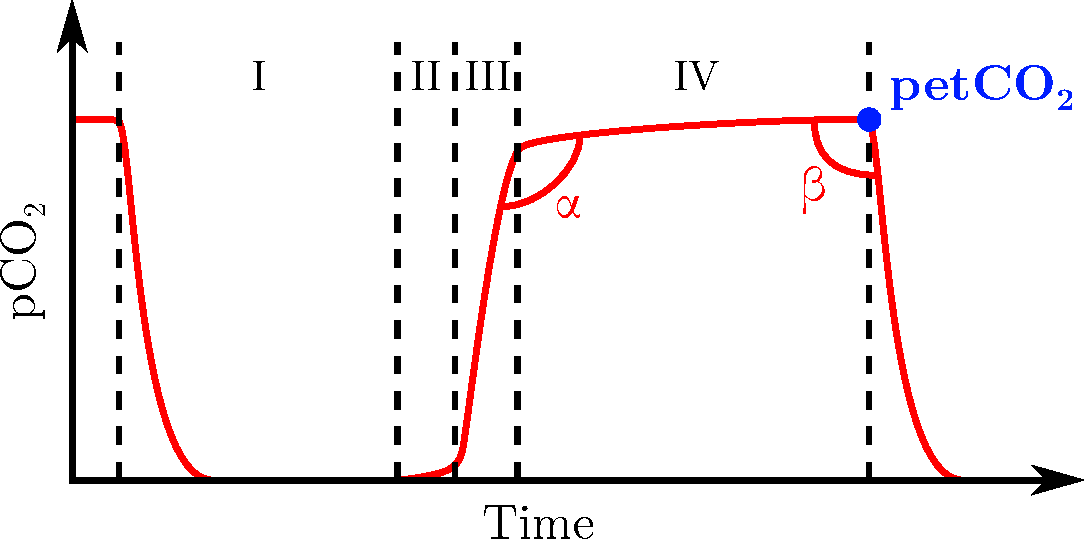
\includegraphics[width=.80\linewidth]{1_main_matter/intro_figures/capnography_principle}
	\caption[Capnography \textit{vs} capnometry.]{A capnogram yields important clinical clues on the state of the patient or quality of their intubation by analysing the different breathing phases---inspiration (I), and expiration: dead-space volume (II), mixed dead-space and alveolar air (III) and alveolar air (IV)---and the two $\alpha$ and $\beta$ angles\cite{capnography_gravenstein, capnography_site}. More narrowly, capnometry is only interested in knowing the more concise end-tidal \gls{pco2} value reached at the end of the plateau (IV): \gls{petco2}.}
	\label{fig:capnometry_principle}
\end{figure}

Capnography is particularly useful in medical practice since it gives information about respiratory airflow, \gls{co2} production and elimination, respiratory quotient, or the quality of endotracheal intubation. It can also be used to detect ventilation / perfusion inadequacy, apnea, \gls{copd} or heart failures\cite{siobal2016, long2017}. For its part, \gls{petco2} has proven to be a reliable proxy for \gls{paco2} under stable haemodynamic conditions, with \gls{petco2} being usually 2--5~mmHg lower than \gls{paco2}\cite{siobal2016}. However, the correlation between \gls{petco2} and \gls{paco2} vanishes in case of elevated physiological dead space or ventilation perfusion mismatch\cite{wagner2015, amaddeo2016}. It can also be difficult to use capnometry on neonates due to the small volume of exhaled air that they produce\cite{hochwald2019}.

Interestingly, Siobal \etal{}\cite{siobal2016} pointed out that, while airway capnometry is often criticised for its inaccuracy as a \gls{paco2} proxy---\eg{} in case of ventilation / perfusion mismatch, elevated dead space, or poor endotracheal placement---the very root causes of this inaccuracy may be characterised by performing a simultaneous \gls{paco2} measurement. In other words, if simultaneous \gls{paco2} and \gls{petco2} measurements are performed in the same patient, discrepancies between the two values may reveal one of the aforementioned issues.

% https://www.sci-hub.se/10.1007/BF03008330 good ref as well!

\subsubsection{Probing Modalities}

Two distinct probing modalities exist for airway capnometry: mainstream or sidestream measurements. In mainstream capnometry, the \gls{co2} sensor is positioned on the main airway of the intubated patient, so that the whole breathed air flow is forced through it. This technique yields instantaneous \gls{petco2} measurement and real-time capnogram plot. Historically, mainstream capnometry has long been criticised because the additional sensor on the patient's airway was bulky, fragile, and led to an additional respiratory dead space. In particular, the bulkiness of mainstream sensors may dislodge the endotracheal tube in young patients\cite{siobal2016, hochwald2019}. In response, recent designs have been improved to become more rugged, compact, and with minimal sampling volume, partially mitigating these drawbacks\cite{jaffe2002, barter2012}.

In contrast, sidestream capnometers consist in a small diameter sampling tube, which continuously aspirates a fraction of the patient's breathed air. The air is then conveyed to an external monitor wherein both the analysis and display functions are performed. Contrary to the mainstream technique, a delay is present between air sampling and the monitoring of its \gls{co2} content\cite{capnography_gravenstein}. Additionally, distortions of the measured capnogram may occur, especially on its more rapidly changing portions, and sidestream-measured \gls{petco2} may be slightly underestimated compared to the mainstream-measured one\cite{balogh2016}.

In practice, airway capnometry is more often than not measured using the infrared absorption of \gls{co2}, either using \gls{ndir} sensors---see Section \ref{subsect:choos:review:ndir}---or photoacoustic sensors---see Section \ref{subsect:choos:review:photoacous}\cite{capnography_gravenstein, siobal2016}. Additionally, colorimetric dye-based sensors---see Section \ref{subsect:choos:review:dye_based}---are also routinely used to assess the correct positioning of endotracheal intubation, although they only provide a qualitative information about the latter, and not a quantitative \gls{ptco2} reading\cite{nakatani1999}.

% Colorimetric attempts, mills? zhao2014

\subsection{Transcutaneous \texorpdfstring{\gls{co2}}{CO2} Sensing}\label{subsect:transcut_capno}

\subsubsection{Clinical Significance}

Transcutaneous \gls{pco2}---\gls{ptco2}---measurements are clinically relevant in two different situations: either as a surrogate for \gls{paco2} in patients with a normal tissue perfusion or as an evaluation tool to measure the \gls{paco2}--\gls{ptco2} gap in patients with an abnormal perfusion\cite{mari2019}.

In patients with normal circulation and peripheral perfusion, \gls{ptco2} correlates well with \gls{paco2} and, as such, may be used in all situations where \gls{paco2} is required\cite{conway2018}. This correlation is particularly influenced by the choice of the measuring site, and by the probe temperature, as disclosed in the next section.

Alternatively, measurements of the \gls{paco2}--\gls{ptco2} gap proved to be a reliable predicator of mortality in case of shock\cite{vallee2019}. In such a view however, a simultaneous measurement of \gls{paco2} is required in addition to \gls{ptco2} monitoring. One may notice the similarity between this technique, and the proposal of Siobal \etal{} for \gls{petco2} mentioned earlier---see Section \ref{subsect:airway_capno_cc}.

\subsubsection{Probing Modalities}

\gls{ptco2} measurements can be performed with the attachment of a transcutaneous probe on the skin by means of a disposable, adhesive mounting ring. The measuring site and sensor temperature depend on what is to be measured: for instance, when searching for a \gls{paco2} surrogate, it is recommended to place the \gls{ptco2} probe at the earlobe with a setpoint temperature above 42~{\degree}C for the best results\cite{conway2018}. However, an elevated skin temperature can be a source of skin burn or thermal injury, especially in the neonates, requiring a frequent change of the probe site\cite{fanconi1996}. A compromise may then be found between skin temperature---and thus site change frequency---and accuracy of the \gls{ptco2} measurement\cite{restrepo2012}. When assessing local perfusion or shock condition---on the contrary---a temperature as low as 37~{\degree}C may be used at the site of interest\cite{vallee2010}. Different temperatures can also be used to assess changes in perfusion as a function of temperature\cite{vallee2019}.

Technically speaking, the \gls{ptco2} is measured by means of a miniaturised \ssel{}---mainly a pH-meter bathing in a bicarbonate solution, see Section \ref{subsect:choos:review:ssel}---which can be heated anywhere in the 37--45~{\degree}C range\cite{mari2019}.

\section{The Need for a Better Alternative}

While the above-mentioned monitors are routinely used in clinical practice, they are not only expensive and invasive, but also bulky and unpractical---for they require frequent external interventions for calibration or sampling purposes. These drawbacks, in addition to turning \gls{pco2} monitors into a coveted resource used sparingly in the hospital, make them unusable outside the clinical setting.

Yet, bringing \gls{pco2} monitors in homes would be highly desirable in a telemonitoring context for home use, reducing the need for hospital visits, and thus the risk of contracting a nosocomial disease. Indeed, if the positive impact of \gls{ptco2} telemonitoring is yet to be demonstrated---for the obvious reason that the corresponding wearable \gls{ptco2} monitor does not exist at the time being---several clinical trials demonstrate the beneficial contribution of telemedicine---\aka{} telehealth---on both patient's outcome and costs of admission in a variety of conditions\cite{steventon2012, kruse2019, yun2018}. Additionally, the outbreak of contagious pandemics---such as COVID-19\cite{garfan2021}---and the rapid development of the health wearable market\cite{dunn2018, yetisen2018, chung2019, dagher2020} may also promote the use of telemonitoring in medical practice. Non-invasive \gls{pao2} and \gls{paco2} monitoring techniques have been an active research field for decades\cite{severinghaus1986_3, severinghaus1986_6, huttmann2014}, but while pulse oximetry proved to be a reliable proxy for \gls{pao2}\cite{nitzan2014, jubran2015}, no satisfactory equivalent exists for \gls{paco2}.

\begin{keypointbox}
	In this context, the development of a non-invasive, low-cost, and portable---if not wearable---biomedical \gls{pco2} monitor appears highly desirable.
\end{keypointbox}

To this end, two main research avenues were explored in the course of this doctoral work: the first one focuses on \gls{co2hb} and proved to be but a dead end, while the second one focuses on transcutaneous \gls{co2} diffusion and led to some successes.

\glsreset{co2hb}
\subsection{The \texorpdfstring{\gls{co2hb}}{Carbamino-Haemoglobin (CO2Hb)} Avenue}

The idea behind the \gls{co2hb} avenue was the following: since \textit{(i)} the oxygenation state of haemoglobin influences its absorption spectrum\cite{prahl1998} and \textit{(ii)} this change in absorption can be detected optically transcutaneously \textit{via} pulse oximetry\cite{nitzan2014, jubran2015}, if \textit{(iii)} a similar change in haemoglobin absorption spectrum can be triggered by the formation of haemoglobin carbamate compounds---\ie{} \gls{co2hb}---then \textit{(iv)} the theory behind pulse oximetry could be applied to the optical transcutaneous determination of the arterial \gls{co2hb} concentration. Then, since an equilibrium exists between this concentration and \gls{paco2}\cite{geers2000}, the latter could be measured non-invasively.

Of course, this train of thought could only succeed if hypothesis \textit{(iii)} were valid. Due to the absence of information on the absorption spectrum of \gls{co2hb} in the literature in 2019, the first part of this doctoral work focused on the spectrophotometry of haemoglobin derivatives---this is the object of Chapter~\ref{chap:co2hb}. In brief, I literally gave my \myblood{} for Science: human haemoglobin was equilibrated with three gases---ambient air, \gls{n2}, and \gls{co2}---and the corresponding absorption spectra were subsequently measured over the 235--1000~nm range. These measurements were published in the Journal of Biomedical Optics in 2020\cite{dervieux2020}, but revealed no differences between \gls{hb} and \gls{co2hb} absorption spectra. Additional fluorescence measurements were also performed, searching for differences in either the excitation or emission spectra of haemoglobin upon \gls{co2} exposition. There again, no major variations could be observed between the fluorescence properties of \gls{hb} and \gls{co2hb}. 

In light of the above, hopes of using a technique akin to pulse oximetry for determining the arterial blood \gls{co2hb} concentration shattered. Subsequently, I reoriented my studies towards transcutaneous \gls{co2} diffusion.

\subsection{The Transcutaneous \texorpdfstring{\gls{co2}}{CO2} Diffusion Avenue}

\subsubsection{Skin Permeability Towards \texorpdfstring{\gls{co2}}{CO2}}

The transcutaneous diffusion of \gls{co2} is at the very core of current \gls{ptco2} monitors. Yet, this phenomenon was poorly documented in the literature, with only a few ageing studies available, which were often performed on a limited number of subjects, and without skin temperature regulation. Since skin permeability towards \gls{co2} is expected to have a major influence on the response time of \gls{ptco2} sensors, I first aimed at better characterising it. In particular, the influence of skin temperature on the latter permeability was vastly unknown. Yet, this temperature / permeability relationship is of crucial importance in the design of a sensor: \textbf{not} heating the skin---or heating it as little as possible---is highly desirable from an energy consumption point-of-view, thus favouring the integration of the said sensor into a wearable. To fill this knowledge gap, a custom sensor was developed and a clinical study was conducted, allowing the measurement of transcutaneous \gls{co2} diffusion rates at the arm and wrist on 40 healthy subjects at five different temperatures. These works are summarised in a 2023 Frontiers in Physiology article\cite{dervieux2023rate}, and are the object of Chapter~\ref{chap:tcco2}.

\subsubsection{Choosing a \texorpdfstring{\gls{co2}}{CO2} Sensing Technique}

Once the rate of diffusion of \gls{co2} through the skin was better known, the next logical step was to choose a \gls{co2} sensing technique for the \gls{ptco2} sensor-to-be. To this end, a comprehensive review of \gls{co2} sensing techniques was performed and published in MDPI's Sensors journal\cite{dervieux2022}. From this review, I concluded that \gls{co2}-responsive fluorescent thin film sensors were a promising avenue. Further research on this sensing modality brought into light the \gls{dlr} sensing scheme---a phase-based approach with sinusoidal illumination power\cite{klimant2001_pap}---for which extensive mathematical derivation were performed. Briefly, those derivations aimed at knowing the reachable accuracy on a \gls{co2} measurement, given the illumination power, measurement duration, and noise levels---they were published in the 
APSIPA Transactions on Signal and Information Processing\cite{dervieux2024phase}. Finally, the chemistry of fluorescence-based \gls{co2} sensing was also modelled, although corresponding experimentations confirming or infirming the presented influence of the different chemicals' concentration are lacking. These different works are compiled in Chapter~\ref{chap:choosing_techno}.

\subsubsection{\texorpdfstring{\gls{co2}}{CO2}-Sensitive Fluorescent Thin Films}

The theoretical aspects of the issue at hand having been sufficiently delineated to allow for initial \invitro{} experiments, the next step was the fabrication of \gls{co2}-sensitive fluorescent thin films, probed through a \gls{dlr} sensing scheme. To this end, the luminescence properties of the selected luminophores were characterised at different temperatures and in the presence / absence of humidity and \gls{co2}. Early bi-layer films showed promising results, having the ability to measure \gls{co2} levels in the 0--10\% range with a response time below 1~min. These results were the object of a short communication at the NEWCAS 2024 conference\cite{dervieux2024newcas}---4-pages paper and lecture---and are reviewed in much more details in Chapter~\ref{chap:thin_film}.

\subsection{Further Research is Needed}

\mfrin{}In spite of the relentless years of meticulous work that were dedicated to this doctoral thesis, many an aspect of the presented research have been left in the shadows. Those are explicitly indicated by the \enquote{further research is needed symbol}---as mentioned in the \hyperref[forechap:foreword]{foreword}---and are reviewed in the concluding chapter---Chapter~\ref{chap:conclusion}. Among them, the study of the influence of skin temperature on the \gls{ptco2} / \gls{paco2} correlation is probably the strongest remaining lock to the development of wearable \gls{ptco2} sensors, as we shall see\dots











